\documentclass{article}
\usepackage{amsmath}
\usepackage{graphicx}
\usepackage{csvrows}

\title{Reviewable Assistant Edits for \LaTeX{} Papers}
\author{Paperd example project}
\date{}

\begin{document}
\maketitle

\begin{abstract}
Writing assistants can propose useful edits, but an edit applied without review can silently change a claim.
We describe a workflow in which every assistant edit is a proposal that the author keeps or discards, and every kept change becomes a revision of the paper.
This paper is the Paperd example project: its history, branches and assistant turns are there to explore, and all numbers in it are illustrative.
\end{abstract}

\section{Introduction}
\label{sec:introduction}

Writing assistants rewrite a paragraph in seconds, and many authors now use one for at least part of a paper~\cite{park2022review}.
Speed is not the problem; accountability is.
When an edit lands directly in the source, nobody decides whether it should, and a changed claim can survive until peer review~\cite{lee2024tracking}.

Version control solves a similar problem for code: every change is recorded and can be compared, restored or merged~\cite{myers1986diff}.
We apply the same idea to papers written in \LaTeX{}~\cite{lamport1994latex}.

Our contribution is a workflow in which assistant output is always a reviewable proposal and every kept change becomes a revision of the paper.
Section~\ref{sec:method} describes the workflow and Section~\ref{sec:results} reports a small illustrative comparison.

\section{Method}
\label{sec:method}

The author writes \LaTeX{} source, and the source is the only version of the paper.
An assistant request names the files or lines it may change.
The assistant answers with a change set: the replaced lines, plus short notes on what changes and why.
Nothing is written until the author keeps the change set.

Figure~\ref{fig:overview} shows the loop: the author drafts, the assistant proposes, and the author decides.

\begin{figure}[t]
\centering
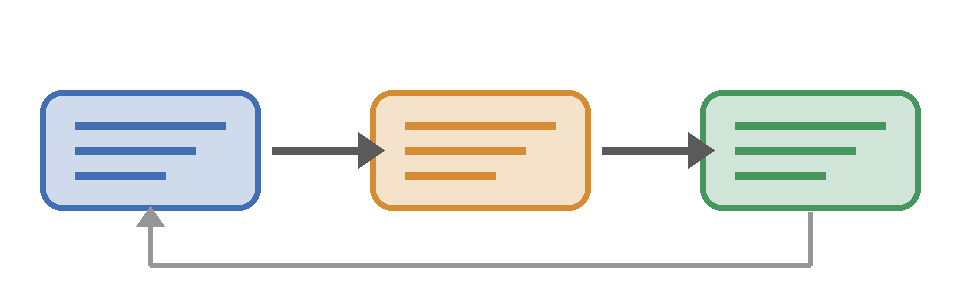
\includegraphics[width=0.9\linewidth]{../Images/overview.png}
\caption{The authoring loop: draft, proposal, decision. A kept proposal becomes a new revision, and the loop starts again.}
\label{fig:overview}
\end{figure}

Each kept change set, like each saved edit, becomes one revision in an append-only history~\cite{haber1991timestamp}.
Named versions mark milestones such as a submission, and draft branches hold changes that are not ready for the main line.

\section{Results}
\label{sec:results}

We compared three settings on the same twelve drafts: manual editing, assistant suggestions applied automatically, and reviewed change sets.
The numbers are illustrative; they live in \texttt{refs/data/results.csv}, and Table~\ref{tab:results} is generated from that file whenever the paper compiles.

\begin{table}[t]
\centering
\caption{Accepted assistant edits, review time per draft and residual errors per page.}
\label{tab:results}
\begin{tabular}{lrrr}
\hline
\csvrows{../refs/data/results.csv}\\
\hline
\end{tabular}
\end{table}

Table~\ref{tab:results} shows that reviewed change sets double the quality of the final draft~\cite{kim2021ledger}.
Reviewers were faster, and errors went down.

The remaining errors were mostly in patch sets that touched several sections at once.

\section{Conclusion}
\label{sec:conclusion}

Treating assistant output as a proposal keeps every change to the paper accountable: each one was reviewed, and each one can be traced to a revision.
Future work will study co-authored papers, where draft branches and reviewed merges matter most.


\bibliographystyle{plain}
\bibliography{references}
\end{document}
